
\chapter{Fundamentals of Accelerator Physics}\label{ch:accelerator_physics_fundamentals}

After the introduction to Hamiltonian mechanics in Chapter~\ref{ch:mathematical_elements}, and the overview of stochastic Hamiltonian systems presented in Chapter~\ref{ch:the_diffusive_framework}, we now turn to the presentation of the fundamental concepts of accelerator physics. In particular, we will introduce the fundamental nomenclature, coordinates, and common approximations and assumptions used in this domain. These concepts will be required to understand the open challenges of non-linear beam dynamics, and how they can be related to known results in the field of stochastic Hamiltonian systems as, as we will see, the field of accelerator physics makes large use of the formalism and results from Hamiltonian mechanics.

It should be noted that the following information is not intended to serve as a comprehensive overview of accelerator physics. For a more detailed introduction to the subject, the reader is directed to Refs.~\cite{Lee:2651939,wiedemann2015particle}, which were consulted in the creation of this chapter. Our focus here is to provide an overview of the specific topics that are propaedeutical for the original contributions of this thesis. 

A particle accelerator is a device that uses electromagnetic fields to accelerate a beam of charged particles, allowing for collisions with a target or another particle beam. These machines can be classified as linear or circular depending on their geometry. This study will focus specifically on circular accelerators.

An important consideration when working with circular particle accelerators is the type of particles that are accelerated, since a charged particle moving along a curved trajectory will lose energy due to synchrotron radiation~\cite{jackson1999classical}. The amount of energy lost per turn in a circular orbit due to synchrotron radiation follows the law~\cite{doi:10.1142/p899}:
\begin{equation}
    U_0 = C_\gamma \beta_0^3\frac{E_0}{\rho}\,,
\end{equation}
where $E_0$ is the energy of the particle, $\beta_0$ the relativistic ratio $v/c$, $\rho$ the radius of the circular orbit, and $C_\gamma = q^2 / 3\epsilon_0(mc^2)^4$ a constant~\cite{sands1970physics} dependent on the particle charge $q$ and mass $m$. Due to the factor $m^{-4}$ in $U_0$, this energy loss factor becomes negligible for hadron beams, but must be taken into account when working with electron beams in circular accelerators. In this research, we will only examine hadron machines and energy scales at which synchrotron radiation can be neglected.

Additionally, this study will focus on single-particle dynamics, which means that the motion of each individual particle in the beam will be considered independent and the repulsive Coulomb force between charges within the beam will be neglected. 

The motion of the particles can be broken down into two components: longitudinal, in the direction of motion along the circumference, and transverse, in the plane normal to the longitudinal motion. These two components are also known, respectively, as synchrotron motion and betatron motion.
The focus of this study will be on the transverse motion of the particles, which, as we will see in this chapter, can be described by means of an ideal integrable Hamiltonian system on which we then add non-linear terms and perturbations to describe the actual beam dynamics.

This non-linear Hamiltonian system describing the betatron motion is the point of departure and motivation for the study of the non-linear betatron motion and the application of the framework presented in the previous chapter, which will be the topic of the following parts and the original contribution of this thesis.

The chapter is organized as follows. In Section~\ref{sec:acc:fernet}, we introduce the Frenet-Serret coordinate system, which is the standard coordinate system used in accelerator physics, and we inspect the Hamiltonian of a charged particle in an electromagnetic field. In Section~\ref{sec:acc:transverse}, we solve the equations of motion in the transverse plane, considering an ideal scenario with only linear components of the magnetic field. Next, in Section~\ref{sec:acc:cs_ellipse}, we define the invariant of the motion, the emittance, which comes from the definition of the Courant-Snyder ellipse. Then, in Section~\ref{sec:non-linear}, we give a brief overview of the effects that arise in betatron motion when considering non-linear terms in the dynamics. In Section~\ref{sec:acc:oneturn}, we introduce the concept of one-turn map, in which the importance of symplectic maps in the context of accelerator physics is shown. In Section~\ref{sec:2:dynamic_aperture}, we present the concept of dynamic aperture and how a Nekhoroshev scaling law emerges from the study of the non-linear dynamics effects on it. Finally, in Section~\ref{sec:acc:longitudinal_dynamics}, we give a brief overview of the fundamental concepts of longitudinal motion, since the modulation effects given by it on the transverse motion will be of specific interest in the Part~\ref{part:dyn} of this thesis, where we will also inspect how modulation effects contribute to the non-linear dynamics of the betatron motion. 


\section{Particle motion and Frenet-Serret coordinate system~\label{sec:acc:fernet}}

The standard choice of coordinates in accelerator physics, which takes advantage of the toroidal symmetry of the circular accelerator, is the Frenet-Serret coordinate system.

Starting from the Cartesian system $(X,\, Y,\, Z)$, centred in the accelerator centre, the Frenet-Serret coordinate system considers as one curvilinear coordinate the path length along the reference orbit $s$, which describes the ideal longitudinal motion of a particle inside the accelerator, and two Cartesian coordinates $x$ and $y$ for the transverse ones. In Fig.~\ref{fig:frenserr}, we illustrate the coordinate system applied to a vector $\vb{r}$.

Mapping the Cartesian system to the Frenet-Serret coordinate system reads:
%
\begin{equation} 
    X = (x+\rho)\cos(\frac{s}{\rho})\,, \qquad Y=y\,, \qquad Z=(x+\rho)\sin(\frac{s}{\rho})\,.
\end{equation}

To keep the particles on a reference orbit of radius $\rho$, a constant magnetic field of intensity $B$ is applied. $\rho$ then is given by the equilibrium between the magnetic force and the centrifugal force. This equilibrium is expressed by the quantity $B\rho$, defined as \textit{beam rigidity}, which corresponds to
\begin{equation}
    B\rho = \frac{p}{e}
    \label{eq:beam_rigidity}
\end{equation}
where $p$ is the momentum of the particle and $e$ its charge.

Starting from this coordinate system, it is possible to achieve a practical Hamiltonian expression for a particle in an accelerator.

\begin{figure}
\centering
\def\svgwidth{0.75\columnwidth}
\import{2_accelerator_physics_fundamentals/figs/}{fernet_nuovo.pdf_tex}
\caption{The Frenet-Serret coordinate system applied to a vector $\vb{r}$ in the starting Cartesian system. The reference orbit represents an ideal trajectory of particles in the accelerator, whose radius of curvature is $\rho$. The coordinate $s$ is measured along the trajectory, while $x$ and $y$ are orthogonal to it.}
\label{fig:frenserr}
\end{figure}

Let us begin from the Hamiltonian of a relativistic charged particle under the effect of an electromagnetic field, which acts on the particle via the Lorentz force. The particles are accelerated, in modulus, by the action of an electric field $\mathbf{E}$ (or by the corresponding scalar potential $\Phi$), and their trajectories are bent, to keep them in the circular reference orbit, by a magnetic field $\mathbf{B}$, which can be expressed via the vector potential $\mathbf{A}$, i.e.\ $\mathbf{B}=\rot\mathbf{A}$.

The Hamiltonian of a relativistic particle under Lorentz force reads
%
\begin{equation}
    \ham = e\Phi + \sqrt{ m^2c^4 + (c\mathbf{p}-e\mathbf{A})^2 }\,. 
\end{equation}
%
We then express the square norm of $(c\mathbf{p}-e\mathbf{A})$ in the Frenet-Serret system of coordinates $(x,\,y,\,s)$, whose metric tensor reads
%
\begin{equation} 
    g_{ij} = \mathrm{diag}\qty(1,\,1,\,1+\frac{x}{\rho})\,, 
\end{equation}
%
which leads to
%
\begin{equation}
    \ham = e\Phi + \sqrt{ m^2c^4 + \frac{(cp_s-eA_s)^2}{(1+x/\rho)^2 } + (cp_x-eA_x)^2+ (cp_y-eA_y)^2}\,.
    \label{eq:ham_process_1}
\end{equation}
%
From now on, it is convenient to treat $s$ as the time coordinate. Consequently, due to canonical coupling, the conjugated momentum $-p_s$ will play the role of a Hamiltonian function $\tilde\ham$. Solving Eq.~\eqref{eq:ham_process_1} for $p_s$, we obtain
%
\begin{equation} 
    \tilde{\ham} = -\qty(1-\frac{x}{\rho})\sqrt{\frac{E^2}{c^2}-m^2c^2-(p_x-eA_x)^2-(p_y-eA_y)^2} - eA_s\,,
\end{equation}
%
where $E=\ham-e\Phi$. We have from special relativity that $E^2/c^2 = p^2 + m^2c^2$,this allows us to rewrite the Hamiltonian as
\begin{equation}
    \tilde{\ham} = -\qty(1-\frac{x}{\rho})\sqrt{p^2-(p_x-eA_x)^2-(p_y-eA_y)^2} - eA_s\,.
\end{equation}

In high-energy circular accelerators, such as those considered for this study,  $p\gg p_x$ and $p\gg p_y$, and the so-called paraxial approximation can be applied. This enables the $\sqrt{1+x}\approx 1+x/2$ expansion for the Hamiltonian, leading to
%
\begin{equation} 
	\tilde\ham = \qty(1+\frac{x}{\rho})\qty[-p + \frac{1}{2p}\qty(p_x^2+p_y^2)] -eA_s\,. 
	\label{eq:hamem}
\end{equation}

It is customary to assume that there is no magnetic field in the longitudinal direction. With this assumption, we only have contributions to the vector potential along $s$, and $A_x=A_y=0$, i.e.\ $\mathbf{B}=(B_x,\,B_y,\,0)$.

The standard approach to evaluating the contribution of the magnetic field to $\tilde\ham$, $eA_s$, consists of expanding the magnetic field in its multipolar components.

From Maxwell's equation $\rot\mathbf{B}=0$, one obtains the Laplace equation $\laplacian\mathbf{A}$, which, for $A_s$, has a general solution that can be expressed in power series as
%
\begin{equation}
	A_s = \Re\sum_{n}\qty[ \frac{k_n + ij_n}{(n+1)}(x+iy)^{n+1}]\, ,%%%TODO::controlla def
	\label{eq:as}
\end{equation}
%
which leads to the corresponding expansion of the magnetic field
\begin{equation}
	B_y + iB_x = \sum_n (k_n + ij_n) (x+iy)^n\,.
\end{equation}
%
The coefficients
\begin{equation}
	k_n = \frac{1}{n!} \pdv[n]{B_y}{x}\eval_{x=y=0}, \qquad 
	j_n = \frac{1}{n!} \pdv[n]{B_x}{y}\eval_{x=y=0} 
\end{equation}
%
are called respectively the \textit{normal} and \textit{skew} $2(n+1)$-polar coefficients of the magnetic field. In accelerator physics, it is customary to consider magnetic elements that generate fields with only one multipolar component. These elements are, in fact, referred to as normal or skew dipoles, quadrupoles, sextupoles, octupoles, etc. Of course, in the case of magnetic field imperfections, several multipolar components can be associated with a single magnet.

%
\section{Transverse motion} \label{sec:acc:transverse}
%

From the Hamiltonian \eqref{eq:hamem}, we can derive the equations of motion of the particle in the transverse plane. We obtain the following
%
\begin{equation}
    \begin{aligned}
        x' &= \qty(1+\frac{x}{\rho})\frac{p_x}{p}\,, &\qquad p_x' &= \frac{p}{\rho}\qty(1+\frac{x}{\rho}) + e\pdv{A_s}{x}\,,\\ % TODO::CHECK
        y' &= \qty(1+\frac{x}{\rho})\frac{p_y}{p}\,, &\qquad p_y' &= e\pdv{A_s}{y}\,.
    \end{aligned}
    \label{eq:ham_motion}
\end{equation}

To obtain an expression for the partial derivatives of $A_s$ as a function of the $x$ and $y$ components of the magnetic field $\mathbf{B}$, we consider the expression of $\curl \mathbf{A}$ in the Frenet-Serret coordinates, which reads
%
\begin{equation}
    \curl \mathbf{A} = \frac{\hat x}{1+x/\rho}\pdv{A_s}{y} - \frac{\hat y}{1+x/\rho}\pdv{A_s}{x} = B_x\hat x + B_y\hat y % TODO::CHECK
\end{equation}
%
as only the $A_s$ component is non-zero. This leads to
%
\begin{equation}
    \pdv{A_s}{x} = -\qty(1+\frac{x}{\rho})B_y\,, \qquad \pdv{A_s}{y} = \qty(1+\frac{x}{\rho})B_x\,,
\end{equation}
%
which, substituted in Eq.~\eqref{eq:ham_motion}, reads
%
\begin{equation} 
    \begin{aligned}
        x' &= \qty(1+\frac{x}{\rho})\frac{p_x}{p}\,, &\qquad p'_x &= \qty(1+\frac{x}{\rho})\qty[ \frac{p}{\rho} - eB_y]\\
        y' &= \qty(1+\frac{x}{\rho})\frac{p_y}{p}\,, &\qquad p'_y &= e\qty(1+\frac{x}{\rho})B_x\,.
    \end{aligned}
\end{equation}
%
Recalling the definition of beam rigidity in Eq.~\eqref{eq:beam_rigidity}, we can rewrite the equations of motion as second-order differential equations using the fact that $p=eB\rho$. This leads to
%
\begin{equation}
    \begin{split}
        x'' &= \frac{1}{\rho} + \frac{x}{\rho^2} + \frac{B_y}{B\rho}\qty(1+\frac{x}{\rho})^2\,,\\
        y'' &= \frac{B_x}{B\rho}\qty(1+\frac{x}{\rho})^2\,.
    \end{split}
    \label{eq:acc_step_1}
\end{equation} 

If we consider only linear terms for the magnetic fields $B_x$ and $B_y$, these equations can be expressed in the form 
\begin{equation}
	z''+K_z(s)z = 0\, ,
    \label{eq:acc_step_2}
\end{equation}
where $z$ stands for $x$ or $y$, and the function $K(s)$ represents the effect of the linear magnetic fields the particle is subject to in the accelerator.  For a circular accelerator of length $L$ the periodic condition $K_z(s)=K_z(s+L)$ holds. This equation with the periodic condition is referred to in the literature as \textit{Hill's equation}.


An Ansatz for the solution of Hill's equation is in the form
\begin{equation}
	z(s)=A\sqrt{\beta_z(s)}\cos\left(\psi_z(s)\right)\,,
	\label{eq:hill_zeta}
\end{equation}
%
\ie a harmonic oscillator where the amplitude $\beta_z(s)$ and phase advance $\psi_z(s)$ depend on $s$. When substituted into Hill's equation, this results in a relation between $\psi_z(s)$ and $\beta_z(s)$, namely
%
\begin{equation}
	\frac{1}{\sqrt{\beta_z(s)}} \dv{s}(\beta_z(s)\psi_z(s)) = 0\,,
\end{equation}
%
which can be solved as
%
\begin{equation}
	\psi_z(s) = \int_0^s \frac{\dd s'}{\beta_z(s')}\,
\end{equation}
%
and a non-linear equation for $\beta_z(s)$:
%
\begin{equation}
	\frac{1}{2}\beta_z\beta_z''-\frac{1}{4}\beta_z'^2+K_z(s)\beta_z^2=1\,.
\end{equation}

The phase advance over the ring is called \textit{tune}:
\begin{equation}
	\nu_z = \frac{1}{2\pi}\oint \frac{\dd s'}{\beta_z(s')}\,.
    \label{eq:tune_def}
\end{equation} 


\section{Courant-Snyder ellipse} \label{sec:acc:cs_ellipse}

As we are interested in the transverse motion of the particle, we want to consider its evolution each time it crosses the position $s=s_0$, i.e.\ we want to consider the Poincaré section of dynamics. At each iteration, we will have a phase advance of $\psi_z$ equal to $2\pi\nu_z$.

It is possible to decouple the envelope dynamics described by $\beta_z(s)$ from the transverse motion of the particles with a coordinate transformation, which leads to the definition of the Courant-Snyder ellipse and other important quantities in accelerator physics.

From Eq.~\eqref{eq:hill_zeta}, we find that $z'(s)$ reads
%
\begin{equation}
	z'(s)=-\frac{z}{\beta_z(s)}\qty(\alpha_z(s)+\tan\psi_z(s))\,
\end{equation}
%
where $\alpha_z=-\beta'_z/2$. We then consider for our coordinate transformation the angular variable $\phi_z=\psi_z$ and the generating function
%
\begin{equation}
	F=\int \dd z\, z' = -\frac{z^2}{2\beta_z}(\alpha_z+\tan\phi_z) \,,
\end{equation}
%
which then yields the canonical action variable $I_z$
%
\begin{equation}
	I_z=\pdv{F}{\phi_z}=\frac{z^2}{2\beta_z}(1+\tan^2\phi_z)=\frac{1}{2\beta_z}\qty[z^2+(\beta_z z'+\alpha_z z)^2]\,.
	\label{eq:jz}
\end{equation}

In the new variables, the Hamiltonian corresponding to Hill's equation
\begin{equation} 
    \ham = \frac{z'^2}{2} + \frac{K_z z^2}{2} \,,
\end{equation}
reduces to the simple expression
\begin{equation}
	\ham(\phi,I,s) = \frac{I}{\beta(s)}\, ,
\end{equation}
which takes into account the derivative $\pdv*{F}{s}$, and from this new Hamiltonian we find that the equation of motion for the variable $\phi_z$ reads $\phi'_z = 1/\beta(s)$. 

We are now interested in making $\phi_z$ proportional to $s$, and removing any dependence on the $\beta$ function in the equations of motion. To achieve this, we define 
\begin{equation}
    \omega_z = \frac{2\pi\nu_z}{L} \,,
\end{equation}
where, we recall, $L$ is the circumference of the accelerator and $\nu_z$ the tune defined in Eq.~\eqref{eq:tune_def}. Then we have the final change of variables $(\phi_z,I_z)\to(\tilde\phi_z, \tilde I_z)$, which is defined by the generating function
%
\begin{equation}
	G(\phi_z,\tilde I_z) = \tilde I_z\qty(\omega_z s - \int_0^s\frac{\dd s'}{\beta(s')})+\phi\tilde I\, ,
\end{equation}
%
which results in the Hamiltonian
%
\begin{equation}
	\ham(\tilde \phi_z,\tilde I_z) = \omega_z \tilde I_z\,,
	\label{eq:harm_ham}
 \end{equation}
%
i.e.\ the well-known Hamiltonian of a harmonic oscillator (note how $I_z$ = $\tilde{I}_z$).

From this final Hamiltonian, one can introduce and operate with normalized Cartesian coordinates 
\begin{equation}
    \hat z=\sqrt{2I_z}\cos\tilde{\phi}_z\,,\quad \hat p_z=\sqrt{2I_z}\sin\tilde{\phi}_z \,,
    \label{eq:2:cart_eq}
\end{equation}
and consequently treat the transverse linear motion on both the $\hat x-\hat p_x$ and $\hat y-\hat p_y$ planes using an intuitive normalized Cartesian Hamiltonian
%
\begin{equation}
	\ham(\hat x,\, \hat p_x,\, \hat y,\, \hat p_y) = \frac{\omega_x}{2}(\hat x^2 +\hat p_x^2) + \frac{\omega_y}{2}(\hat y^2+\hat p_y^2)\, .
	\label{eq:linham}
\end{equation}
%

\begin{figure}
    \centering
    \def\svgwidth{0.75\columnwidth}
    \import{2_accelerator_physics_fundamentals/figs/}{ellisse.pdf_tex}
    \caption{The Courant-Snyder ellipse $\gamma z^2 + 2\alpha zz' + \beta z'^2=2I_z$. The area enclosed by the ellipse is equal to $2\pi I_z$. }
    \label{fig:coursnyd}
\end{figure}


The Hamiltonian of Eq.~\eqref{eq:linham} describes circular trajectories in decoupled phase spaces $(\hat x,\,\hat p_x)$ and $(\hat y\,, \hat p_y)$. Moreover, there are two corresponding action variables, namely,
\begin{equation}
    I_x = \frac{\hat x^2 +\hat p_x^2}{2}\,, \quad I_y=\frac{\hat y^2+\hat p_y^2}{2} \,,
\end{equation}
can be defined. $I_x$ and $I_y$ follow the standard definition of the trajectory area divided by $2\pi$ and are conserved. However, for historical reasons, the value $2I_z$ is called \text{Courant-Snyder invariant}.

Following its definition in the physical coordinates $(z,\, z')$, given in Eq.~\eqref{eq:jz}, it is possible to draw the constant-$I$ surfaces in the $(z,z')$ phase space, as in Fig.~\ref{fig:coursnyd}, which correspond to concentric ellipses, as the expanded form reads:
%
\begin{equation}
I_z = \frac{1}{2\beta_z}\qty[z^2 + (\alpha z + \beta z'))^2] = \frac{1}{2}\qty(\gamma z^2 + 2\alpha z z' + \beta z'^2)\,, \end{equation}
%
where we have defined $\gamma=(1+\alpha^2)/\beta$. The area of the ellipse is equal to $2\pi I_z$, and is conserved at any value of $s$. It can be observed, finally, how the $(z,z')\to(\hat z,\hat p_z)$ coordinate transformation modifies the physical coordinates ellipses into circles with the same area, from which their name \textit{``normalized coordinates''}.

A single particle following the linear transverse dynamics will have its own constant Courant-Snyder invariant. When, instead, we want to consider a beam distribution, a standard property, called \textit{emittance} is defined as the average of the Courant-Snyder invariant:
\begin{equation}
    \eps_z = \av{I_z} \,.
\end{equation}
The emittance is related to the second moments of the beam distribution in $(\hat z,\hat p_z)$. In fact, averaging over $I_z$ and $\phi_z$ in the definitions of $\hat z$ and $\hat p_z$ given in Eq.~\eqref{eq:2:cart_eq}, we obtain the following
%
\begin{equation}
	\av{\hat z^2} = \beta_z \eps_z, \qquad \av{\hat p_z^2}=\gamma_z \eps_z, \qquad \av{\hat z\,\hat p_z}=-\alpha_z\eps_z\,,
\end{equation}
%
from there, using the definition of $I_z$ yields
\begin{equation}
	\eps_z = \sqrt{ \av{\hat z^2}\av{\hat p_z^2} - \av{\hat z \, \hat p_z}^2 }\,.
\end{equation}

The beam emittance can then be considered as the average Courant-Snyder invariant of a distribution or as the area (up to a $2\pi$ factor) of the orbit of the RMS particle of the beam. A useful implication of this is that a Gaussian beam distribution in $(\phi_z,\,I_z)$ coordinate assumes the following practical form
%
\begin{equation}
\rho_z = \frac{1}{\eps_z}\exp(-\frac{I_z}{\eps_z})\,.
\end{equation}
%

\section{Non-linear beam dynamics}\label{sec:non-linear}

The transverse dynamics we treated so far takes into consideration only the effects of a linear magnetic field (we recall the step between Eq.~\eqref{eq:acc_step_1} and Eq.~\eqref{eq:acc_step_2}, where we dropped all non-linear terms for the magnetic fields $B_x$ and $B_y$), so that this approach takes into account only the elements generated by a set of ideal dipole and quadrupole magnets.

To include higher-order terms of the magnetic field power series, it is possible to include non-linear terms directly into Hill's Hamiltonian. This can be done to represent both the unavoidable higher-order magnet imperfections inside the accelerator machine, or to represent explicit sextupolar and octupolar elements, which one might want to include in the accelerator lattice. 

As Hill's Hamiltonian is equivalent to two uncoupled harmonic oscillators, non-linear components can be included in the Hamiltonian as anharmonic perturbation. We start by considering higher-order terms $n \ge 2$ of the power series $A_s$ in Eq.~\eqref{eq:as}, and we perform the change of variables $(x,\,y) \to (\hat x, \hat y)$. We then see that the non-linear part of the Hamiltonian reads:
%
\begin{equation}
    \ham_\text{nlin}(\hat x, \hat p_x, s) = \Re \sum_{n\ge 2} \qty[\frac{k_n(s) + ij_n(s)}{(n+1)} \left(\sqrt{\beta_x(s)}\ \hat x + i\sqrt{\beta_y(s)}\ \hat y\right)^n]\,.
\end{equation}  

To approximate this expression to a simpler form, we introduce the quantity $\beta(s)=\beta_y(s)/\beta_x(s)$, and its value $\overline{\beta}$ averaged over the accelerator circumference, which reads
\begin{equation}
    \overline{\beta} = \oint \dd s\, \frac{\beta_y(s)}{\beta_x(s)} \,.
\end{equation}
We can now substitute the strengths $k_n(s)$ and $j_n(s)$ (which, we recall, represent the effect of a normal or a skew magnetic field $(2n+2)$) with the integrated coefficients $K_n$, $J_n$, which will be scaled by the value of $\beta_x(s)$ and $\beta_y(s)$, that is, we weight the integral average with the envelope value of the beam where the magnetic elements are placed. These coefficients read
%
\begin{equation} 
	K_n = \oint \dd s\, k_n(s) \beta_x^{\frac{n}{2}}(s)\,,\qquad
	J_n = \oint \dd s\, j_n(s) \beta_x^{\frac{n}{2}}(s)\,.
\end{equation} 
%
With this notation, the non-linear Hamiltonian has the simpler form
% 
\begin{equation} \ham_\text{nlin}(\hat x, \hat p_x) = \Re \sum_{n\ge 2} \qty[\frac{K_n + iJ_n}{(n+1)} (\hat x + i\overline{\beta}^{1/2} \hat y)^n]\,.\end{equation}

From this Hamiltonian, one can for example write a simple beam model with one degree of freedom and normal multipoles
\begin{equation}
	\ham(\hat x,\hat p) = \omega \frac{\hat x^2 + \hat p^2}{2} + \sum_{n>2} K_n \frac{x^{n+1}}{(n+1)}\, ,
	\label{eq:hamxp_nl}
\end{equation}
such a simple model can be used to understand many phenomena caused by non-linear effects.

In an accelerator, non-linear effects can be used to represent either unwanted elements, such as magnet imperfections, or to represent specifically added elements generating a non-linear magnetic field, such as sextupoles and octupoles. These components can be introduced into an accelerator lattice to correct specific unwanted effects, like \textit{chromaticity}, i.e.\ the fact that particles with different momentum are differently focused by quadrupoles. Chromaticity, specifically, can be controlled by the introduction of sextupole magnets. Another important source of non-linearities is space charge effects and \textit{beam-beam interaction}, caused by the electromagnetic interaction of charged particles with other charged particles, respectively, in the same or in another beam during collisions.

The introduction of non-linear elements in a circular accelerator is the cause of three main effects~\cite{herr}: amplitude-dependent detuning, excitation of non-linear resonances, and reduction of the dynamic aperture. We will present the first two phenomena very briefly and focus a little more on the core characteristics of the last one.

\subsubsection{Amplitude-dependent detuning}

Adding non-linear elements has the inevitable consequence of making the tune, i.e.\ the rotation frequency of the harmonic oscillator, an amplitude-dependent function. In the linear Hamiltonian~\eqref{eq:linham}, the frequency $\Omega$ is given by
\begin{equation}
	\Omega = \pdv{\ham}{I} = \omega\,,
\end{equation}
where, we recall, $I=(\hat x^2 + \hat p^2)/2$. The tune $\Omega$ is constant at any $I$, therefore, all particles have the same tune.

If we now add an octupolar component to the Hamiltonian, that is, an $n=3$ element of the power series in Eq.~\ref{eq:hamxp_nl}, the new Hamiltonian is
\begin{equation}
	\ham = \omega \frac{\hat x^2 + \hat p^2}{2} + \frac{K_3}{5} x^4 = \omega I + \frac{K_3}{5} I^2 \cos^4\phi\, .
\end{equation}

Averaging over the angular variable $\phi$, one obtains
\begin{equation}
	\av{\ham} = \omega I + \frac{3}{40}K_3 I^2,
\end{equation}
%
and
%
\begin{equation}
	\Omega(I) = \pdv{\av{\ham}}{I} = \omega + \frac{3K_3}{20} I\,.
\end{equation}
There is now a linear dependence of the tune on the action $I$, and each particle will have a different rotation frequency depending on its amplitude.

The averaging approach used here to obtain an expression of the amplitude detuning highlights only the first-order effects in the frequency. For more complex Hamiltonians, describing multiple non-linear components, deriving a complete analytical expression of the detuning is not always a trivial task.

It is possible to numerically evaluate the amplitude-dependent detuning in single-particle tracking simulations, as the tune can be measured by performing a numerical estimate of the fundamental frequency of the orbit. We will present the topic of tune evaluation later in Chapter~\ref{ch:overview_of_dynamic_indicators}, in the context of dynamic indicators, as tune determination is the foundation for consolidated tools in accelerator physics like Frequency Map Analysis.

\subsubsection{Non-linear resonances}

If the tunes $\omega_x$ and $\omega_y$ satisfy a 1\textsc{d} or 2\textsc{d} resonance condition, the non-linear magnetic field can eventually lead to severe particle loss. A theoretical approach to this phenomenon is presented in~\cite{Bazzani:262179, wilson}.

When the frequency $\omega_x$ or $\omega_y$ is close to a 1\textsc{d} resonant condition $n\omega_z / 2\pi \in \mathbb{Q}$, according to the Poincaré-Birkhoff theorem, presented in Section~\ref{subsec:poincare-birkhoff}, a chain of islands with extra fixed points appears. These islands, in regular accelerator operations, may reduce the dynamic aperture (for which the definition is given in Section~\ref{sec:2:dynamic_aperture}) and, close to separatrices, cause the onset of chaotic motion. When a resonance is crossed due to small, undesired variations of the magnetic field, which cause oscillations of $\omega_x$ and $\omega_y$ values, a growth in beam emittance may be observed~\cite{Guignard:185921}, affecting beam lifetime.

Other than 1\textsc{d} resonances, in a system with two degrees of freedom, one can have a 2\textsc{d} resonant condition between the $\omega_x$ and $\omega_y$ frequencies, i.e.\ $m\omega_x+n\omega_y = 2\pi\ell$, with $\ell \in \mathbb{Q}$. Only difference resonances ($m>0$, $n<0$) are stable, although they contribute to the motion coupling between the two planes, while sum resonances (when $m$ and $n$ have the same signs) result in unstable motion.

\begin{figure}
	\centering
	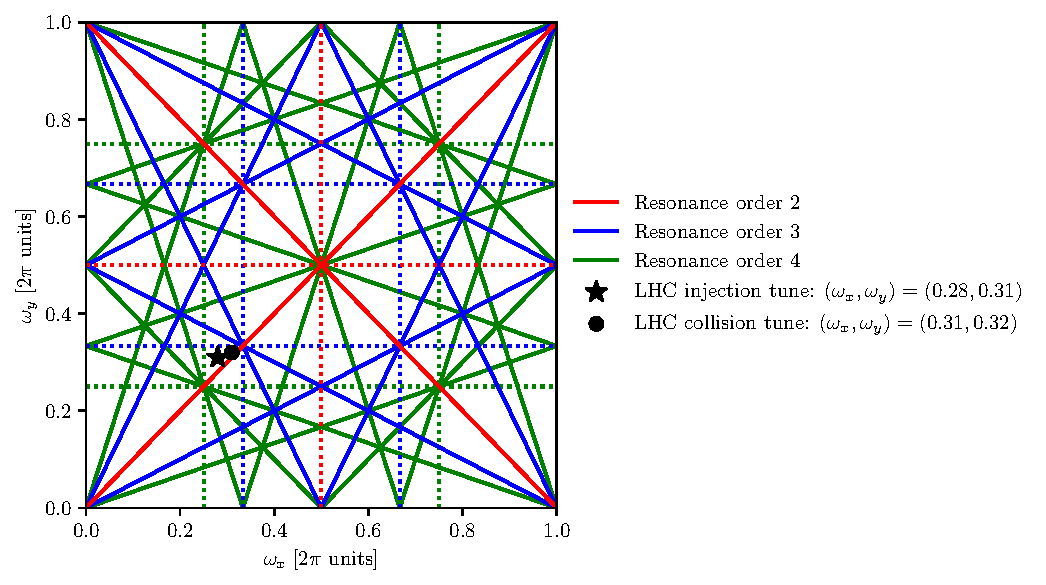
\includegraphics[width=.85\textwidth]{2_accelerator_physics_fundamentals/figs/tune_space.pdf}
	\caption{Resonance diagram in the $(\omega_x,\,\omega_y)$ space up to order $4$, that is, $|m|+|n| = 4$. The resonances are evaluated on the fractional part of $\omega_x$ and $\omega_y$. Dotted lines represent 1\textsc{d} resonances, continuous lines represent 2\textsc{d} resonances. The two characteristic working fractional tunes for the LHC are also reported on the resonance diagram.}
	\label{fig:res}
\end{figure}

The possible 1\textsc{d} and 2\textsc{d} resonances (up to order $4$) are represented by lines in the $(\omega_x, \omega_y)$ diagram in Fig.~\ref{fig:res}, where different colours show the resonance order. As higher-order resonances are generally weaker than lower-order ones, the accelerator working point should be selected far from the main resonances; the LHC does so by operating at fractional tunes $(\omega_x, \omega_y)=(0.28, 0.31)$ during injection and $(\omega_x, \omega_y)=(0.31, 0.32)$ during collisions~\cite{Benedikt:823808}. Note that, in the accelerator literature, frequencies and tunes are reported in units of $2\pi$. 

\section{One-turn maps} \label{sec:acc:oneturn}

A standard tool in accelerator physics to inspect the transverse dynamic of a particle in an accelerator magnetic lattice is one-turn maps. A one-turn map \(\mathrm{M}\) is the Poincaré map of the circular accelerator in section $(s = s_0)$, and is given by composing single-element maps:
\begin{equation}
	\mathrm{M} = \mathrm{M}^{(L)} \circ \mathrm{M}^{(L - 1)} \circ \cdots \circ \mathrm{M}^{(2)} \circ \mathrm{M}^{(1)} \,,
\end{equation}
where each $\mathrm{M}^{(i)}$ represents an element along the circular accelerator lattice, which might be, for example, a drift space without magnets, a dipole bending magnet, a quadrupole, or a higher order magnetic element. 

The map \(\mathrm{M}\) transforms the phase space coordinates \(\vb{\hat x} = (\hat x, \hat p_x, \hat y, \hat p_y)\) of a particle into new coordinates \(\vb{x}'\) which correspond to the particle after one full turn (see Fig.~\ref{fig:poincare}).

In this framework, the effect of each magnetic element on the phase coordinates of the beam can be written, in an analogy with geometrical optics, as the action of a $4\times4$ matrix on the coordinate vector. This matrix corresponds to the symplectic flow of the Hamiltonian for a given magnetic field.

When considering only the linear components in the magnetic lattice, the resulting Poincaré map for $\vb{\hat x}$ reads as a decoupled harmonic oscillator
%
\begin{equation} 
	\begin{pmatrix}
		\hat x \\ \hat p_x \\ \hat y \\ \hat p_y 
	\end{pmatrix}_{n+1}
	=
	\begin{pmatrix}
		\cos\omega_x & \sin\omega_x & 0 & 0 \\
		-\sin\omega_x & \cos\omega_x & 0 & 0 \\
		0 & 0 &\cos\omega_y & \sin\omega_y \\
		0 & 0 &-\sin\omega_y & \cos\omega_y
	\end{pmatrix}
	\begin{pmatrix}
		\hat x \\ \hat p_x \\ \hat y \\ \hat p_y 
	\end{pmatrix}_{n}\,.
\end{equation}

In general, it is not possible to compute exactly the transfer map of a non-linear element. Therefore, approximation techniques become necessary. The standard approach that is used in standard tracking codes such as SixTrack~\cite{sixtrack}, is the \textit{one-kick approximation}, i.e.\ it is assumed that the higher-order polynomial effects on the magnetic potential are all located at a precise position $s_l$ and act with a $\delta(s - s_l)$ potential.

The main advantages of this approximation is the fact that the resulting one-turn map $\mathrm{M}$ maintains its symplectic character and enables efficient tracking. This approximation holds when the higher-order magnetic contributions are small in length.

A one-turn map with a single non-linear contribution, added 
with the one-kick approximation at $s = s_0$, will then read  
\begin{equation}
	\begin{pmatrix}
		\hat x \\ \hat p_x \\ \hat y \\ \hat p_y 
	\end{pmatrix}_{n+1}
	=
	R(\omega_x,\omega_y)
	\begin{pmatrix}
		\hat x \\ \hat p_x + \Re \sum_r\frac{K_r + iJ_r}{r}(\hat x+ i\sqrt{\beta}\hat y)^r \\ \hat y \\ \hat p_y - \Im \sum_r\frac{K_r + iJ_r}{r}(\hat x+ i\sqrt{\beta}\hat y)^r  
	\end{pmatrix}_{n}\,,
\end{equation}
where now the $\beta$ term, which also appears in the definition of $K$ and $J$ is evaluated at $s=s_0$ due to the one-kick approximation.

This shape of the map inspired the investigation of 2\textsc{d} and 4\textsc{d} maps in the form of
\begin{equation}
	\begin{pmatrix}
		\hat{\mathbf{x}} \\ \hat{\mathbf{p}}  
	\end{pmatrix}_{n+1}
	=
	\mathrm{R}(\bm\omega)
		\begin{pmatrix}
			\hat{\mathbf{x}} \\ \hat{\mathbf{p}} + \mathbf{f}(\hat{\mathbf{x}})
	\end{pmatrix}_{n} \,,
	\label{eq:henonlike}
\end{equation}
which are referred to as \textit{Hénon-like maps}, due to the well-known map introduced in Ref.~\cite{henon}:
%
\begin{equation}
	\begin{pmatrix}
		\hat x \\ \hat p_x
	\end{pmatrix}_{n+1}
	=
	R(\omega)
		\begin{pmatrix}
			\hat x \\ \hat p_x + \hat x^2
	\end{pmatrix}_{n} \,.
	\label{eq:simplehenon}
\end{equation}

These models, despite their simplicity, already manifest multiple features that are observed in a beam under non-linear magnetic fields and have been used in multiple studies to investigate such features in the context of accelerator physics, especially in the context of dynamic aperture measurements~\cite{PhysRevE.53.4067, invlog}. These maps were also used as a fundamental building block for the application of Normal Form theory to betatron motion~\cite{Bazzani:262179}.

\section{Dynamic aperture}
\label{sec:2:dynamic_aperture}

As shown before, the linear transverse motion can be described as an always stable harmonic oscillator with two degrees of freedom. When instead non-linearities are introduced, the stability of the system is affected and the occurrence of hyperbolic points and resonances makes the motion of various initial conditions chaotic, eventually leading to their loss as they hit the mechanical aperture of the accelerator.

In this scenario, where the region of stable motion in the phase space is affected by the non-linear elements in the Hamiltonian, we can introduce the concept of \textit{Dynamic Aperture} (DA), as the extent of the phase-space region where stable motion occurs up to a given number of turns $N$.

A complete discussion of the definition of DA, its computation, and its accuracy can be found in Refs.~\cite{PhysRevE.53.4067, invlog}, which provide a fundamental starting point on the topic. In the context of single-particle tracking, DA is defined over the number of turns $N$ as the radius of a hypersphere whose volume is equal to the volume of the phase space where stable motion occurs up to $N$ turns. Note how this definition neglects the island of stability, which might be given by the Poincaré-Birkhoff theorem.

\begin{comment}
A formal definition of DA reads as follows
\begin{definition}
	(Dynamic Aperture). Let \(A\) be the physical aperture of the accelerator, i.e.\ the subset of the phase space that can be confined in the beam pipe, and let \(\mathrm{M}\) be the one-turn map of the magnetic lattice. We define the formal DA as
	\begin{equation}
		\mathcal{D}(N)=\bigcap_{n=0}^N \mathrm{M}^{(n)}(A)\,.
	\end{equation}
	We recall that \(\mathrm{M}\) has an elliptic fixed point at the origin.

	Let \(z\in \mathcal{D}(N)\), we define \(\Pi_X z=x\) as the projection of \(z\) on the configuration space; the set
	\begin{equation}
		\Pi_X\mathcal{D}(N)
	\end{equation}
	may have a very complex topology so that it is convenient to compute the convex envelope of the connected component containing the origin, i.e.\ we neglect the islands of stability which might be given by the Poincaré-Birkhoff theorem.

	To define the measure of such a component, we proceed as follows: for each direction \(\hat \phi\in S^d\)  (where \(S^d\) is the unit sphere or a sector of the unit sphere) in the configuration space, we define
	\begin{equation}
	    R(\hat \phi; N)=\lambda_\ast\quad s.t.\quad \lambda \hat\phi\in \Pi_X \mathcal{D}(N)\quad \forall \quad \lambda\in[0,\lambda_\ast]\,,
	    \label{eq:ideal-R}
	\end{equation}
	so that we can finally define the Dynamic Aperture as
	\begin{equation}
        DA(N)=\frac{1}{\mu(S^d)}\int_{S^d} R(\hat \phi; N)d\hat\phi\,,
        \label{eq:formal_da}
	\end{equation}
	where \(\mu\) is the volume measure in the configuration space.
	\label{def:dynamic_aperture}
\end{definition}
\end{comment}

The value of (N) must be adapted for a suitable time frame. In a mathematical sense, stable motion implies a bounded motion for \(N\rightarrow\infty\). In our accelerator context, stable motion and particle stability can be linked to a maximum number of turns \(N_{\text{max}}\), where the value of \(N_{\text{max}}\) is set on the basis of the specific application under consideration, e.g.\ in the LHC a standard 10-hour luminosity fill, which corresponds to, using the revolution frequency of \(\SI{11.245}{\kHz}\)~\cite{Benedikt:823808}, \(\sim 10^9\) turns.

A consolidated numerical method for evaluating the DA in four-dimensional symplectic mappings that model betatron motion is presented in Ref.~\cite{PhysRevE.53.4067}.

Let us operate on a 4\textsc{d} phase space on which we have a one-turn map \(\mathrm{M}\). If we consider an ensemble of initial conditions defined on a polar grid (\(x=r\cos\phi, p_x=0, y=r\sin\phi, p_y=0\)), \(0\leq\phi\leq\pi/2\), where \(x,y\) are expressed in units \(\sigma_x, \sigma_y\), i.e.\ nominal beam emittance units, and we track them for up to \(N_{\text{max}}\) turns to assess their stability, then we can define DA as:
\begin{equation}
	DA(N) = \frac{2}{\pi}\int_0^{\pi/2} r(\phi;N)\,d\phi \equiv \langle r(\phi;N)\rangle
	\label{eq:dynamic_aperture_numerical}
\end{equation}
where \(r(\phi;N)\) is the last stable amplitude, i.e.\ \(x^2 + y^2 < r_{\mathrm{max}}\) for every iteration of \(\mathrm{M}\), not disconnected from the origin for up to \(N\) turns in the direction \(\phi\). %We can say that \(r\) is the computable version of the `ideal' \(R(\phi;N)\) given in Eq.~\eqref{eq:ideal-R}.

In addition to this consolidated ``radial scan'' method, other techniques have been studied to improve the convergence speed of numerical DA measurements, such as the one presented in Ref.~\cite{vanderveken:ipac2022-mopost047}, where a Support Vector Machine algorithm is employed to perform an optimized sampling and border detection of the stable region of the phase space.

\subsection{Dynamic aperture scaling laws}

Simulating entire sets of initial conditions on different one-turn maps is a computationally intense task that becomes unsustainable when considering extremely high \(N_{\text{max}}\) values or complex symplectic tracking models\footnote{Researches like~\cite{invlog} present simulations in $N_\text{max}\sim 10^6-10^7$, while instead it would be necessary to reach values \(\sim 10^9\).}. Moreover, the multipolar components of the various superconducting magnets are known only with limited precision, so one has to perform parametric studies to consider different realizations of the magnetic lattice. Because of these reasons, realistic timescales in tracking simulation are still out of reach for proper accelerator physics research.

This limitation motivated the search for a robust model for the time dependence of DA, as such a model could offer insights into the long-term evolution of DA by extrapolating short-term tracking simulation data. The most recent developments on the topic of DA scaling laws can be found in~\cite{Bazzani:2019csk} and references therein.

The models presented in~\cite{Bazzani:2019csk} are based on the Nekhoroshev theorem. Previous models formulated scaling laws using both the KAM theorem and the Nekhoroshev estimate, theorizing the presence of a stable core with KAM tori and an increasingly chaotic region where Nekhoroshev-like estimates for stability times apply. However, such models presented some internal discrepancies, such as the possibility to fit non-physical parameters or the strong correlation between free parameters~\cite{Giovannozzi:2018wmm,Giovannozzi:2018igq}, motivated the usage of a scaling law exclusively based on the Nekhoroshev theorem. This is justified by the fact that the condition for the applicability of the stability-time estimate provided by the Nekhoroshev theorem is more general than the existence conditions of the KAM tori.

In this context, the Nekhoroshev theorem can be used to provide an estimate of the number of turns $N(r)$ for which the orbit of an initial condition with amplitude $r$ remains bounded. The estimate has a functional form that reads:
\begin{equation}
    \frac{N(r)}{N_0} = \sqrt{\frac{r}{r_\ast}} \exp\left[\left(\frac{r_\ast}{r}\right)^{\frac{1}{\kappa}}\right]\,.
    \label{eq:specific_nek_estimate}
\end{equation}
A more generalized form of this estimate reads
\begin{equation}
    \frac{N(r)}{N_0} = \left(\frac{r}{r_\ast}\right)^{\lambda} \exp\left[\left(\frac{r_\ast}{r}\right)^{\frac{1}{\kappa}}\right]\,.
\end{equation}

From this working hypothesis, the latest scaling law inspected in~\cite{Bazzani:2019csk}, based on inverting the functional form of the Nekhoroshev estimate, reads:
\begin{equation}
	DA(N) = \frac{\rho_\ast}{\left[-2 \mathrm{e} \lambda \mathcal{W}_{-1}\left(-\frac{1}{2 \mathrm{e} \lambda}\left(\frac{\rho_*}{6}\right)^{1 / \kappa}\left(\frac{8}{7} N\right)^{-1 /(\lambda \kappa)}\right)\right]^\kappa}\,,
	\label{eq:giova_interpolation}
\end{equation}
where $\mathcal{W}$ is the Lambert-$\mathcal{W}$ function~\cite{Corless1996}. The free parameters in this equation are $\rho_\ast$, $\kappa$, and possibly $\lambda$, unless it is set at $1/2$. The parameter $\rho_\ast$ is related to the Nekhoroshev parameters in Eq.~\eqref{eq:specific_nek_estimate} with the following relation:
\begin{equation}
    \rho_\ast = \left(\frac{\kappa}{2e}\right)^{-\kappa} r_\ast \,.
\end{equation}

% Another thing we are interested in is the establishment of a direct link between the DA and the expected beam lifetime in a synchrotron, in order to transform a DA interpolating law into an expected beam-quality model. The approach proposed in~\cite{giovannozzi2012proposed} considers an initial 2\textsc{d} Gaussian distribution for a beam
% \begin{equation}
% 	\rho_G(x,y) = \frac{1}{2\pi\sigma_x\sigma_y}e^{-\left(\frac{x^2}{2\sigma_x^2}+\frac{y^2}{2\sigma_y^2}\right)}
% 	\label{eq:initial_gaussian_beam}
% \end{equation}
% then, transforming~\eqref{eq:initial_gaussian_beam} to polar coordinates and applying the DA definition~\eqref{eq:dynamic_aperture_numerical}, i.e.\ assuming that all particles with starting amplitude beyond \(DA(N)\) are lost after \(N\) turns, we can directly compute the evolution of beam intensity \(N_b\) with the following equation
% \begin{equation}
% 	\frac{N_b(N)}{N_b(1)} = 1 - \int_{DA(N)}^{+\infty} e^{-\frac{r^2}{2}} r \, dr = 1 - e^{-\frac{D^2(N)}{2}}
% 	\label{eq:measuring_da}
% \end{equation}
% with \(DA(N) \xrightarrow[N \to 0]{} +\infty \). This last equation represents a starting point for building the direct connection we are looking for, and also allows us to establish some experimental procedures for evaluating DA from beam losses in a circular accelerator.

\section{Fundamentals of longitudinal dynamics} \label{sec:acc:longitudinal_dynamics}

Although the focus of this work is on the transverse beam dynamics, it is important to include an essential presentation of the core concepts behind the longitudinal dynamics, i.e., the theory describing synchrotron oscillations. A particle that exhibits a longitudinal displacement with respect to the reference trajectory, or that has a longitudinal momentum different from the reference, will also manifest a different transverse dynamics, with a mechanism called \textit{syncro-betatron coupling}. The main effects of syncro-betatron coupling can be represented as a turn-dependent \textit{modulation} of transverse tunes.

In high-energy circular accelerators, the acceleration of particles is achieved via the use of time-varying electromagnetic fields. The accelerating fields are generated in dedicated straight elements, called RF cavities. In these cavities, a high-frequency accelerating voltage $V$ is generated along the longitudinal direction with a specified angular frequency $\omega_{\mathrm{rf}}$, and reads
\begin{equation}
    V=V_0 \sin \left(\omega_{\mathrm{rf}} t+\phi_s\right),
\end{equation}
where $V_0$ is the amplitude of the RF voltage and $\phi_s$ is a phase factor.

When the momentum of a particle in an accelerator changes, its revolution frequency $f$ also changes, following a relation that reads:
\begin{equation}
    \frac{\mathrm{d} f}{f}=\left(\frac{1}{\gamma_r^2}-\alpha_{\mathrm{p}}\right) \frac{\mathrm{d} p}{p}\,,
\end{equation}
where $\gamma_r$ is the Lorentz factor and $\alpha_{\mathrm{p}}$ is referred to as the momentum compaction factor, it depends on the lattice, and it is the ratio between the relative orbit difference (given by the different trajectory in the magnetic lattice) and the relative momentum error
\begin{equation}
    \alpha_p = \frac{1}{C}\dv{\Delta C}{\delta} = \frac{1}{C} \oint \frac{{D}(s)\,\mathrm{d}s}{\rho}\,,
\end{equation}
where $C$ is the path length of the reference orbit, $\delta$ is the fractional off-momentum $\Delta p / p$, and ${D}(s)$ is the dispersion function~\cite{Lee:2651939}, which quantifies the change in orbit effects given by fractional differences in momentum $\delta$ along the various components of the magnetic lattice.

From this equation we can distinguish two separate regimes. At $\left(\gamma_r^{-2}<\alpha_p\right)$, which corresponds to low energies, the frequency of the revolution decreases with increasing momentum. At $\left(\gamma_r^{-2}>\alpha_{\mathrm{p}}\right)$, which corresponds to high energies, it increases. The energy corresponding to $\gamma_{\mathrm{tr}}=1 / \sqrt{\alpha_{\mathrm{p}}}$ is referred to as \textit{transition energy}, as it delimits the two regimes. %We will now focus on the regime below the transition energy.

Taking into account a particle with longitudinal phase $\phi=\phi_s$, momentum $p_0$, and revolution period $T_0$, we will refer to this particle as \textit{synchronous particle}. When designing an accelerator, we must have that the angular frequency of the RF cavity must match the frequency of the synchronous particle. Such a requirement reads as follows
\begin{equation}
    \omega_{\mathrm{rf}}=h \omega_0\,,
\end{equation}
where $\omega_0=\beta_0 c / R_0$ is the angular revolution frequency of the synchronous particle with $\beta_0$, $R_0$ denoting the speed and average orbit radius of the synchronous particle, respectively, and $h$ is an integer known as the harmonic number, which also represents the number of equally spaced synchronous positions that can be exhibited along the circular accelerator.

The energy gained by the synchronous particle in each passage through the RF cavity will then be dependent on $\phi_s$ and equal to $\Delta E=e V_0 \sin \left(\phi_s\right)$. However, in a real beam, we will have a spread of particles with different particle momenta, and each of these particles will follow a different orbit, due to the different interactions with the accelerator magnetic lattice. Due to such off-momentum orbit and speed differences, each of these off-momentum particles will have a different revolution frequency than the reference particle and, therefore, will receive a different $\Delta E$ from the RF cavity.

In the regime below the transition energy $\gamma < \gamma_\text{tr}$, a higher-momentum particle will arrive at the RF cavity ahead of the synchronous particle, i.e.\ $\left(\phi_1<\phi_s\right)$, and will have a lower $\Delta E$ than the synchronous particle, causing a decrease in its phase. On the contrary, a particle with a lower momentum will arrive at the RF cavity behind the synchronous particle, i.e.\ $\left(\phi_2>\phi_s\right)$, and have a higher $\Delta E$ than the synchronous particle, which causes instead an increase in its phase. In the regime above the transition energy $\gamma > \gamma_\text{tr}$, the correlation between the difference in $\Delta E$ and phase variation is inverted.

In Fig.~\ref{fig:long_1}, we show a simple scheme for an accelerating synchronous particle for both regimes. We can observe how the two regimes require the synchronous particle to be at a different RF voltage phase to achieve a stable accelerating regime. In Fig.~\ref{fig:long_2}, instead, we show a sketch of a stationary synchronous particle above the transition energy, along with the resulting potential well described by the RF voltage frequency.

\begin{figure}[p]
    \centering
    \def\svgwidth{0.85\columnwidth}
    \import{2_accelerator_physics_fundamentals/figs/}{longitudinal_bis.pdf_tex}
    \caption{Sketch of the different $V$ provided at particles with different $\phi$ for an accelerating synchronous particle, and consequent phase evolution respectively in the regime below transition energy (left, $\gamma < \gamma_\text{tr}$), and in the regime above transition energy (right, $\gamma > \gamma_\text{tr}$). $\phi_s$ and $\phi'_s$ represent the synchronous particle phase at $\gamma < \gamma_\text{tr}$ and $\gamma > \gamma_\text{tr}$, respectively. $\phi_1$ and $\phi_2$ are respectively the phase of a particle with higher and lower longitudinal momentum, the same goes for $\phi'_1$ and $\phi'_2$. The frequency of the RF voltage provides a restoring force towards $\phi_s$, causing a different effect on the phase depending on the value of $\gamma$.}
    \label{fig:long_1}

    \vspace{\floatsep}
    
    \def\svgwidth{0.85\columnwidth}
    \import{2_accelerator_physics_fundamentals/figs/}{longitudinal_ter.pdf_tex}
    \caption{Sketch of the different $V$ provided at particles with different $\phi$ for a stationary synchronous particle above transition energy. The synchronous particle $\phi_s$ receives no energy from the RF voltage, while particles at different phase receive a restoring force towards $\phi_s$. The frequency of the RF voltage (black curve) describes a potential well with the minimum corresponding to the synchronous particle (red curve).}
    \label{fig:long_2}
\end{figure}

The resulting motion in the longitudinal plane, related to the potential well given by the RF voltage frequency, is called \textit{synchrotron motion}, which is characterized by \textit{synchrotron oscillations}. The fractional off-momentum deviation is then defined as
\begin{equation}
    \delta=\frac{\Delta p}{p_0}=\frac{\omega_0}{\beta^2 E} \frac{\delta E}{\omega_0} \,.
\end{equation}

From this we then obtain the equations of motion for the longitudinal variables.
\begin{equation}
    \begin{aligned}
    \frac{\mathrm{d} \delta}{\mathrm{d} t} &=\frac{\omega_0}{2 \pi \beta^2 E} e V_0\left[\sin (\phi)-\sin \left(\phi_s\right)\right] \,, \\
    \frac{\mathrm{d} \phi}{\mathrm{d} t} &=h \omega_0 \eta \delta,
    \end{aligned}
\end{equation}
where $\eta$ is the \textit{slip factor} and reads
\begin{equation}
    \eta=\frac{\Delta \omega / \omega_0}{\Delta p / p_0} \,,
\end{equation}
and assumes positive values below the transition energy and negative values above the transition energy.

When considering small oscillation amplitudes, we can treat the synchrotron motion as that of a harmonic oscillator, where we consider the linearized equation of motion in the variable $\Delta \phi=\phi-\phi_s$. This approach leads to the differential equation
\begin{equation}
    \frac{\mathrm{d}^2}{\mathrm{d} t^2} \Delta \phi-\frac{h \omega_0^2 e V \eta \cos \left(\phi_s\right)}{2 \pi \beta^2 E} \Delta \phi=0 \,.
\end{equation}

We then have the following condition for phase stability
\begin{equation}
    \eta \cos \left(\phi_s\right)<0 .
\end{equation}
The separatrix given by the equations of motion delimits different stable areas in the phase space. The area of stable motion is called \textit{RF bucket}. %In Fig.~\ref{} we show a simple schetch of an RF bucket, along with the separatrix orbit that delimits it.

Particles with small off-momentum deviations undergo a synchrotron oscillation during their orbit. This oscillation periodically alters the magnetic lattice effect on their transverse dynamics as well, leading to what we referred to as syncro-betatron coupling.

In the context of particle tracking simulations (which also include longitudinal dynamics, will be a 6\textsc{d} tracking), different sets of longitudinal variables can be used along the transverse ones~\cite{xsuite:physics}:
\begin{equation}
    \begin{aligned}
    \xi &= s \frac{\beta}{\beta_0}-\beta c t \,,\quad& \tau &= \frac{s}{\beta_0}-c t \,,\quad& \zeta &= s-\beta_0 c t \,;\\
    \delta &= \frac{p-p_0}{p_0} \,,\quad& p_\tau &= \frac{1}{\beta_0} \frac{E-E_0}{E_0} \,,\quad& p_\zeta &= \frac{1}{\beta_0^2} \frac{E-E_0}{E_0}\,; \\
    \end{aligned}
\end{equation}
where variables in the same columns are canonically conjugate.
The different variables can be easily related to each other:
\begin{equation}
    \begin{aligned}
    &\xi=\beta \tau=\frac{\beta}{\beta_0} \zeta \,,\\
    &\delta=\beta p_\tau+\frac{\beta-\beta_0}{\beta_0}=\beta \beta_0 p_\zeta+\frac{\beta-\beta_0}{\beta_0} \,.
    \end{aligned}
\end{equation}

